% A custom target mark painted in two separate PGF path operations.
\documentclass[border=2pt]{standalone}
\usepackage{tikz}
\usetikzlibrary{arrows.meta,plotmarks,positioning}

\pgfdeclareplotmark{review target}{
  \pgfpathcircle{\pgfpointorigin}{\pgfplotmarksize}
  \pgfusepathqfillstroke
  \pgfpathmoveto{\pgfqpoint{-\pgfplotmarksize}{0pt}}
  \pgfpathlineto{\pgfqpoint{\pgfplotmarksize}{0pt}}
  \pgfpathmoveto{\pgfqpoint{0pt}{-\pgfplotmarksize}}
  \pgfpathlineto{\pgfqpoint{0pt}{\pgfplotmarksize}}
  \pgfusepathqstroke
}

\begin{document}
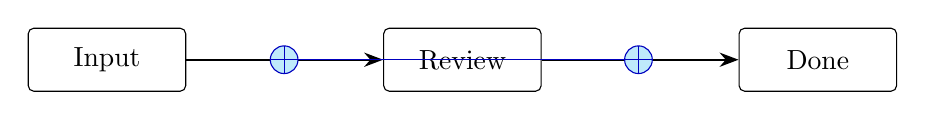
\begin{tikzpicture}[
  stage/.style={draw,rounded corners=2pt,minimum width=2cm,minimum height=8mm},
  flow/.style={-{Stealth[length=2.4mm]},thick}
]
  \node[stage] (input) {Input};
  \node[stage,right=2.5cm of input] (review) {Review};
  \node[stage,right=2.5cm of review] (done) {Done};
  \draw[flow] (input) -- (review);
  \draw[flow] (review) -- (done);
  \draw[blue!75!black,fill=cyan!25,mark size=5pt]
    plot[mark=review target] coordinates {(2.25,0) (6.75,0)};
\end{tikzpicture}
\end{document}
